\PassOptionsToPackage{unicode=true}{hyperref} % options for packages loaded elsewhere
\PassOptionsToPackage{hyphens}{url}
%
\documentclass[10pt,]{article}
\usepackage{lmodern}
\usepackage{amssymb,amsmath}
\usepackage{ifxetex,ifluatex}
\usepackage{fixltx2e} % provides \textsubscript
\ifnum 0\ifxetex 1\fi\ifluatex 1\fi=0 % if pdftex
  \usepackage[T1]{fontenc}
  \usepackage[utf8]{inputenc}
  \usepackage{textcomp} % provides euro and other symbols
\else % if luatex or xelatex
  \usepackage{unicode-math}
  \defaultfontfeatures{Ligatures=TeX,Scale=MatchLowercase}
\fi
% use upquote if available, for straight quotes in verbatim environments
\IfFileExists{upquote.sty}{\usepackage{upquote}}{}
% use microtype if available
\IfFileExists{microtype.sty}{%
\usepackage[]{microtype}
\UseMicrotypeSet[protrusion]{basicmath} % disable protrusion for tt fonts
}{}
\IfFileExists{parskip.sty}{%
\usepackage{parskip}
}{% else
\setlength{\parindent}{0pt}
\setlength{\parskip}{6pt plus 2pt minus 1pt}
}
\usepackage{hyperref}
\hypersetup{
            pdfborder={0 0 0},
            breaklinks=true}
\urlstyle{same}  % don't use monospace font for urls
\usepackage[margin=1in]{geometry}
\usepackage{color}
\usepackage{fancyvrb}
\newcommand{\VerbBar}{|}
\newcommand{\VERB}{\Verb[commandchars=\\\{\}]}
\DefineVerbatimEnvironment{Highlighting}{Verbatim}{commandchars=\\\{\}}
% Add ',fontsize=\small' for more characters per line
\usepackage{framed}
\definecolor{shadecolor}{RGB}{248,248,248}
\newenvironment{Shaded}{\begin{snugshade}}{\end{snugshade}}
\newcommand{\AlertTok}[1]{\textcolor[rgb]{0.94,0.16,0.16}{#1}}
\newcommand{\AnnotationTok}[1]{\textcolor[rgb]{0.56,0.35,0.01}{\textbf{\textit{#1}}}}
\newcommand{\AttributeTok}[1]{\textcolor[rgb]{0.77,0.63,0.00}{#1}}
\newcommand{\BaseNTok}[1]{\textcolor[rgb]{0.00,0.00,0.81}{#1}}
\newcommand{\BuiltInTok}[1]{#1}
\newcommand{\CharTok}[1]{\textcolor[rgb]{0.31,0.60,0.02}{#1}}
\newcommand{\CommentTok}[1]{\textcolor[rgb]{0.56,0.35,0.01}{\textit{#1}}}
\newcommand{\CommentVarTok}[1]{\textcolor[rgb]{0.56,0.35,0.01}{\textbf{\textit{#1}}}}
\newcommand{\ConstantTok}[1]{\textcolor[rgb]{0.00,0.00,0.00}{#1}}
\newcommand{\ControlFlowTok}[1]{\textcolor[rgb]{0.13,0.29,0.53}{\textbf{#1}}}
\newcommand{\DataTypeTok}[1]{\textcolor[rgb]{0.13,0.29,0.53}{#1}}
\newcommand{\DecValTok}[1]{\textcolor[rgb]{0.00,0.00,0.81}{#1}}
\newcommand{\DocumentationTok}[1]{\textcolor[rgb]{0.56,0.35,0.01}{\textbf{\textit{#1}}}}
\newcommand{\ErrorTok}[1]{\textcolor[rgb]{0.64,0.00,0.00}{\textbf{#1}}}
\newcommand{\ExtensionTok}[1]{#1}
\newcommand{\FloatTok}[1]{\textcolor[rgb]{0.00,0.00,0.81}{#1}}
\newcommand{\FunctionTok}[1]{\textcolor[rgb]{0.00,0.00,0.00}{#1}}
\newcommand{\ImportTok}[1]{#1}
\newcommand{\InformationTok}[1]{\textcolor[rgb]{0.56,0.35,0.01}{\textbf{\textit{#1}}}}
\newcommand{\KeywordTok}[1]{\textcolor[rgb]{0.13,0.29,0.53}{\textbf{#1}}}
\newcommand{\NormalTok}[1]{#1}
\newcommand{\OperatorTok}[1]{\textcolor[rgb]{0.81,0.36,0.00}{\textbf{#1}}}
\newcommand{\OtherTok}[1]{\textcolor[rgb]{0.56,0.35,0.01}{#1}}
\newcommand{\PreprocessorTok}[1]{\textcolor[rgb]{0.56,0.35,0.01}{\textit{#1}}}
\newcommand{\RegionMarkerTok}[1]{#1}
\newcommand{\SpecialCharTok}[1]{\textcolor[rgb]{0.00,0.00,0.00}{#1}}
\newcommand{\SpecialStringTok}[1]{\textcolor[rgb]{0.31,0.60,0.02}{#1}}
\newcommand{\StringTok}[1]{\textcolor[rgb]{0.31,0.60,0.02}{#1}}
\newcommand{\VariableTok}[1]{\textcolor[rgb]{0.00,0.00,0.00}{#1}}
\newcommand{\VerbatimStringTok}[1]{\textcolor[rgb]{0.31,0.60,0.02}{#1}}
\newcommand{\WarningTok}[1]{\textcolor[rgb]{0.56,0.35,0.01}{\textbf{\textit{#1}}}}
\usepackage{longtable,booktabs}
% Fix footnotes in tables (requires footnote package)
\IfFileExists{footnote.sty}{\usepackage{footnote}\makesavenoteenv{longtable}}{}
\usepackage{graphicx,grffile}
\makeatletter
\def\maxwidth{\ifdim\Gin@nat@width>\linewidth\linewidth\else\Gin@nat@width\fi}
\def\maxheight{\ifdim\Gin@nat@height>\textheight\textheight\else\Gin@nat@height\fi}
\makeatother
% Scale images if necessary, so that they will not overflow the page
% margins by default, and it is still possible to overwrite the defaults
% using explicit options in \includegraphics[width, height, ...]{}
\setkeys{Gin}{width=\maxwidth,height=\maxheight,keepaspectratio}
\setlength{\emergencystretch}{3em}  % prevent overfull lines
\providecommand{\tightlist}{%
  \setlength{\itemsep}{0pt}\setlength{\parskip}{0pt}}
\setcounter{secnumdepth}{5}
% Redefines (sub)paragraphs to behave more like sections
\ifx\paragraph\undefined\else
\let\oldparagraph\paragraph
\renewcommand{\paragraph}[1]{\oldparagraph{#1}\mbox{}}
\fi
\ifx\subparagraph\undefined\else
\let\oldsubparagraph\subparagraph
\renewcommand{\subparagraph}[1]{\oldsubparagraph{#1}\mbox{}}
\fi

% set default figure placement to htbp
\makeatletter
\def\fps@figure{htbp}
\makeatother

\usepackage{amsthm}
\usepackage{amsmath}
\usepackage{amssymb}
\usepackage{verbatim}
\usepackage{hyperref}
\usepackage[T1]{fontenc}
\usepackage[utf8]{inputenc}
\usepackage[icelandic]{babel}
\hypersetup{colorlinks,allcolors=blue}
\usepackage{enumerate}
\usepackage{lastpage}
\usepackage[shortlabels]{enumitem}
\usepackage{fancyhdr}
\pagestyle{fancy}
\fancyhf{}
\fancyhead[R]{Þórarinn Jónmundsson}
\fancyhead[C]{Dæmi um skýrslu}
\fancyhead[L]{Sumarverkefni}
\fancyfoot[L]{Háskóli Íslands}
\fancyfoot[R]{\thepage}
\usepackage{float}
\usepackage{algorithm}
\usepackage{algorithmicx}
\usepackage{algpseudocode}
\usepackage{caption}
\usepackage[sectionbib]{chapterbib}
\usepackage{booktabs}
\usepackage{longtable}
\usepackage{array}
\usepackage{multirow}
\usepackage{wrapfig}
\usepackage{float}
\usepackage{colortbl}
\usepackage{pdflscape}
\usepackage{tabu}
\usepackage{threeparttable}
\usepackage{threeparttablex}
\usepackage[normalem]{ulem}
\usepackage{makecell}
\usepackage{xcolor}

\author{}
\date{\vspace{-2.5em}}

\begin{document}

%\begin{titlepage}
%\thispagestyle{empty}
\begin{center}
\LARGE{\textbf{Sumarverkefni}}\\
\vspace*{2\baselineskip}
\Large{\textbf{Dæmi um skýrslu}}
\end{center}
% \end{titlepage}
\thispagestyle{empty}
\newpage

\hypertarget{inngangur}{%
\section{Inngangur}\label{inngangur}}

Stutt sýnidæmi um hvernig skal skrifa skýrslu í RMarkdown með version-control.

\hypertarget{uppsetning}{%
\subsection{Uppsetning}\label{uppsetning}}

Fyrst skal:

\begin{enumerate}
\def\labelenumi{\arabic{enumi}.}
\item
  Búa til nýtt repo á github (helst með README).
\item
  Í RStudio:

  \begin{itemize}
  \item
    File -\textgreater{} New Project -\textgreater{} Version Control
  \item
    Copy/Paste slóðina á repo (í mínu tilfelli (\url{https://github.com/thorj/verkferli}))
  \end{itemize}
\end{enumerate}

Þá ætti repo-ið að birtast á tölvunni ykkar. Það inniheldur bara README skrá en við bætum í það.

\begin{enumerate}
\def\labelenumi{\arabic{enumi}.}
\setcounter{enumi}{2}
\item
  Stofna viðeigandi möppur (t.d. \texttt{scripts}, \texttt{data}, \texttt{img}, etc).
\item
  Prufa að commit og push á git í gegnum RStudio (líka hægt í terminal en þetta er ``noob-vænna'')
\end{enumerate}

Getið notað ssh eða venjulegt log-in. Sjá nánar \href{https://happygitwithr.com/}{hér}.

\hypertarget{suxfdniduxe6mi}{%
\section{Sýnidæmi}\label{suxfdniduxe6mi}}

Ef það er verið að vinna með stór gagnasett er tímasóun að vinna allt í einni Rmd skrá sem þarf að endurkeyra kóðann í hvert skipti sem hún er prjónuð. Betra að búta vinnsluna niður í nokkrar skriptur með vel skilgreind hlutverk. Til dæmis:

\begin{enumerate}
\def\labelenumi{\arabic{enumi}.}
\item
  \texttt{settings.R}: Hleður inn öllum viðeigandi R pökkum og yfirskrifar default \texttt{ggplot2} stillingar.
\item
  \texttt{simulate\_binomial.R}: Skripta sem býr til ``stórt'' gagnasett með óskilvirkum kóða. Ef hann væri í Rmd skránni tæki nokkrar mín að prjóna skjalið í hvert sinn.
\item
  \texttt{binomial\_wrangl.R}: Eftir að það er búið að búa til gögnin með \texttt{simulate\_binomial.R} þá eru allar myndir og töflur gerðar með þessari skriptu.
\end{enumerate}

\hypertarget{luxfdsing}{%
\subsection{Lýsing}\label{luxfdsing}}

Til að búa til stutt sýnidæmi voru 50000 tvíkosta strengir hermdir og geymdir ásamt summu strengjanna. Algengustu 10 strengirnir voru fundnir ásamt hlutfalli þeirra af heildarfjölda allra strengja. Strengina ásamt hlutföllum þeirra má sjá í töflu \ref{tab:strings} og á mynd \ref{fig:stringplt}.

\begin{table}[!h]

\caption{\label{tab:unnamed-chunk-3}\label{tab:strings} Hér má sjá 10 algengustu strengina ásamt hlutfalli þeirra.}
\centering
\begin{tabular}[t]{rc}
\toprule
\textbf{Strengur} & \textbf{Hlutfall}\\
\midrule
000000000000 & 0.35118\\
000000001000 & 0.03400\\
100000000000 & 0.03384\\
001000000000 & 0.03268\\
000000010000 & 0.03250\\
000100000000 & 0.03230\\
000010000000 & 0.03210\\
000000000010 & 0.03190\\
010000000000 & 0.03184\\
000001000000 & 0.03166\\
\bottomrule
\end{tabular}
\end{table}

\begin{figure}[H]

{\centering 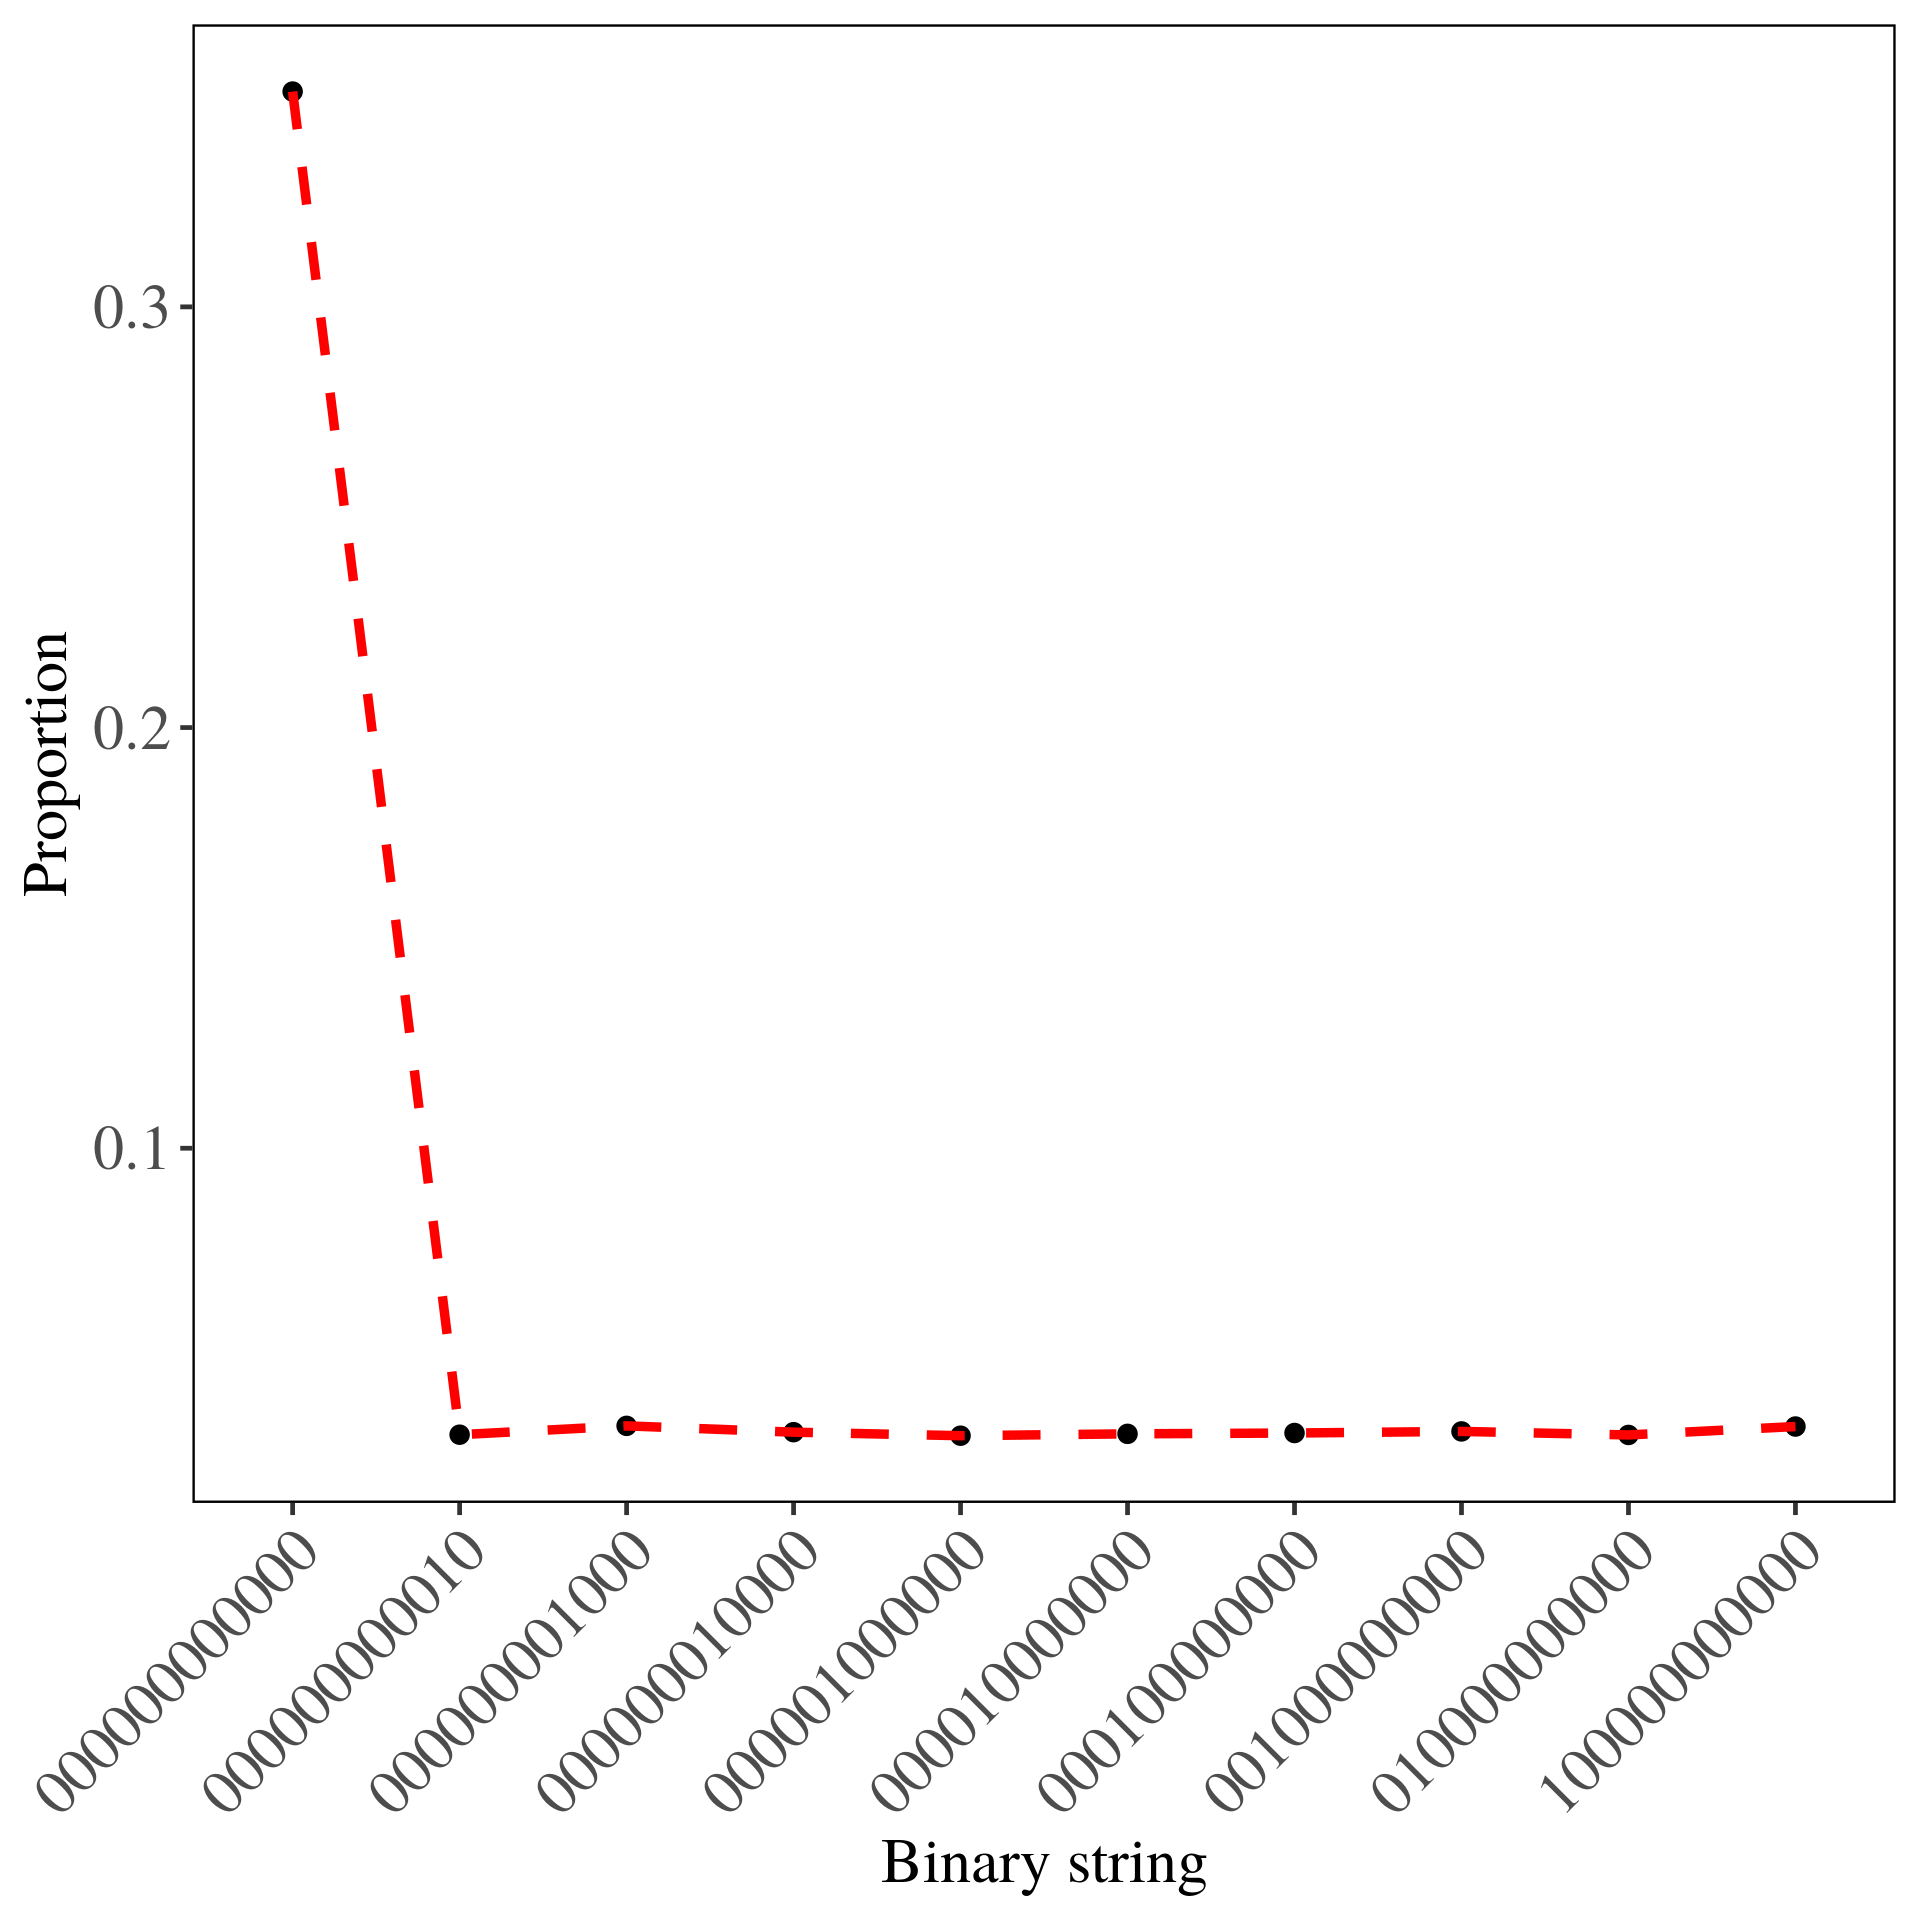
\includegraphics[width=1\linewidth]{img/prop_plt} 

}

\caption{Tíu algengustu strengirnir ásamt hlutfalli þeirra. Hér sést greinilega að 0-strengurinn er algengastur sem er afleiðing að því að strengirnir voru hermdir með litlu $p$.}\label{fig:stringplt}
\end{figure}

Það var líka áhugi fyrir því að teikna stöplarit (súlurit?) af summu strengjanna. Hana má sjá á mynd \ref{fig:sumplt}.

\begin{figure}[H]

{\centering 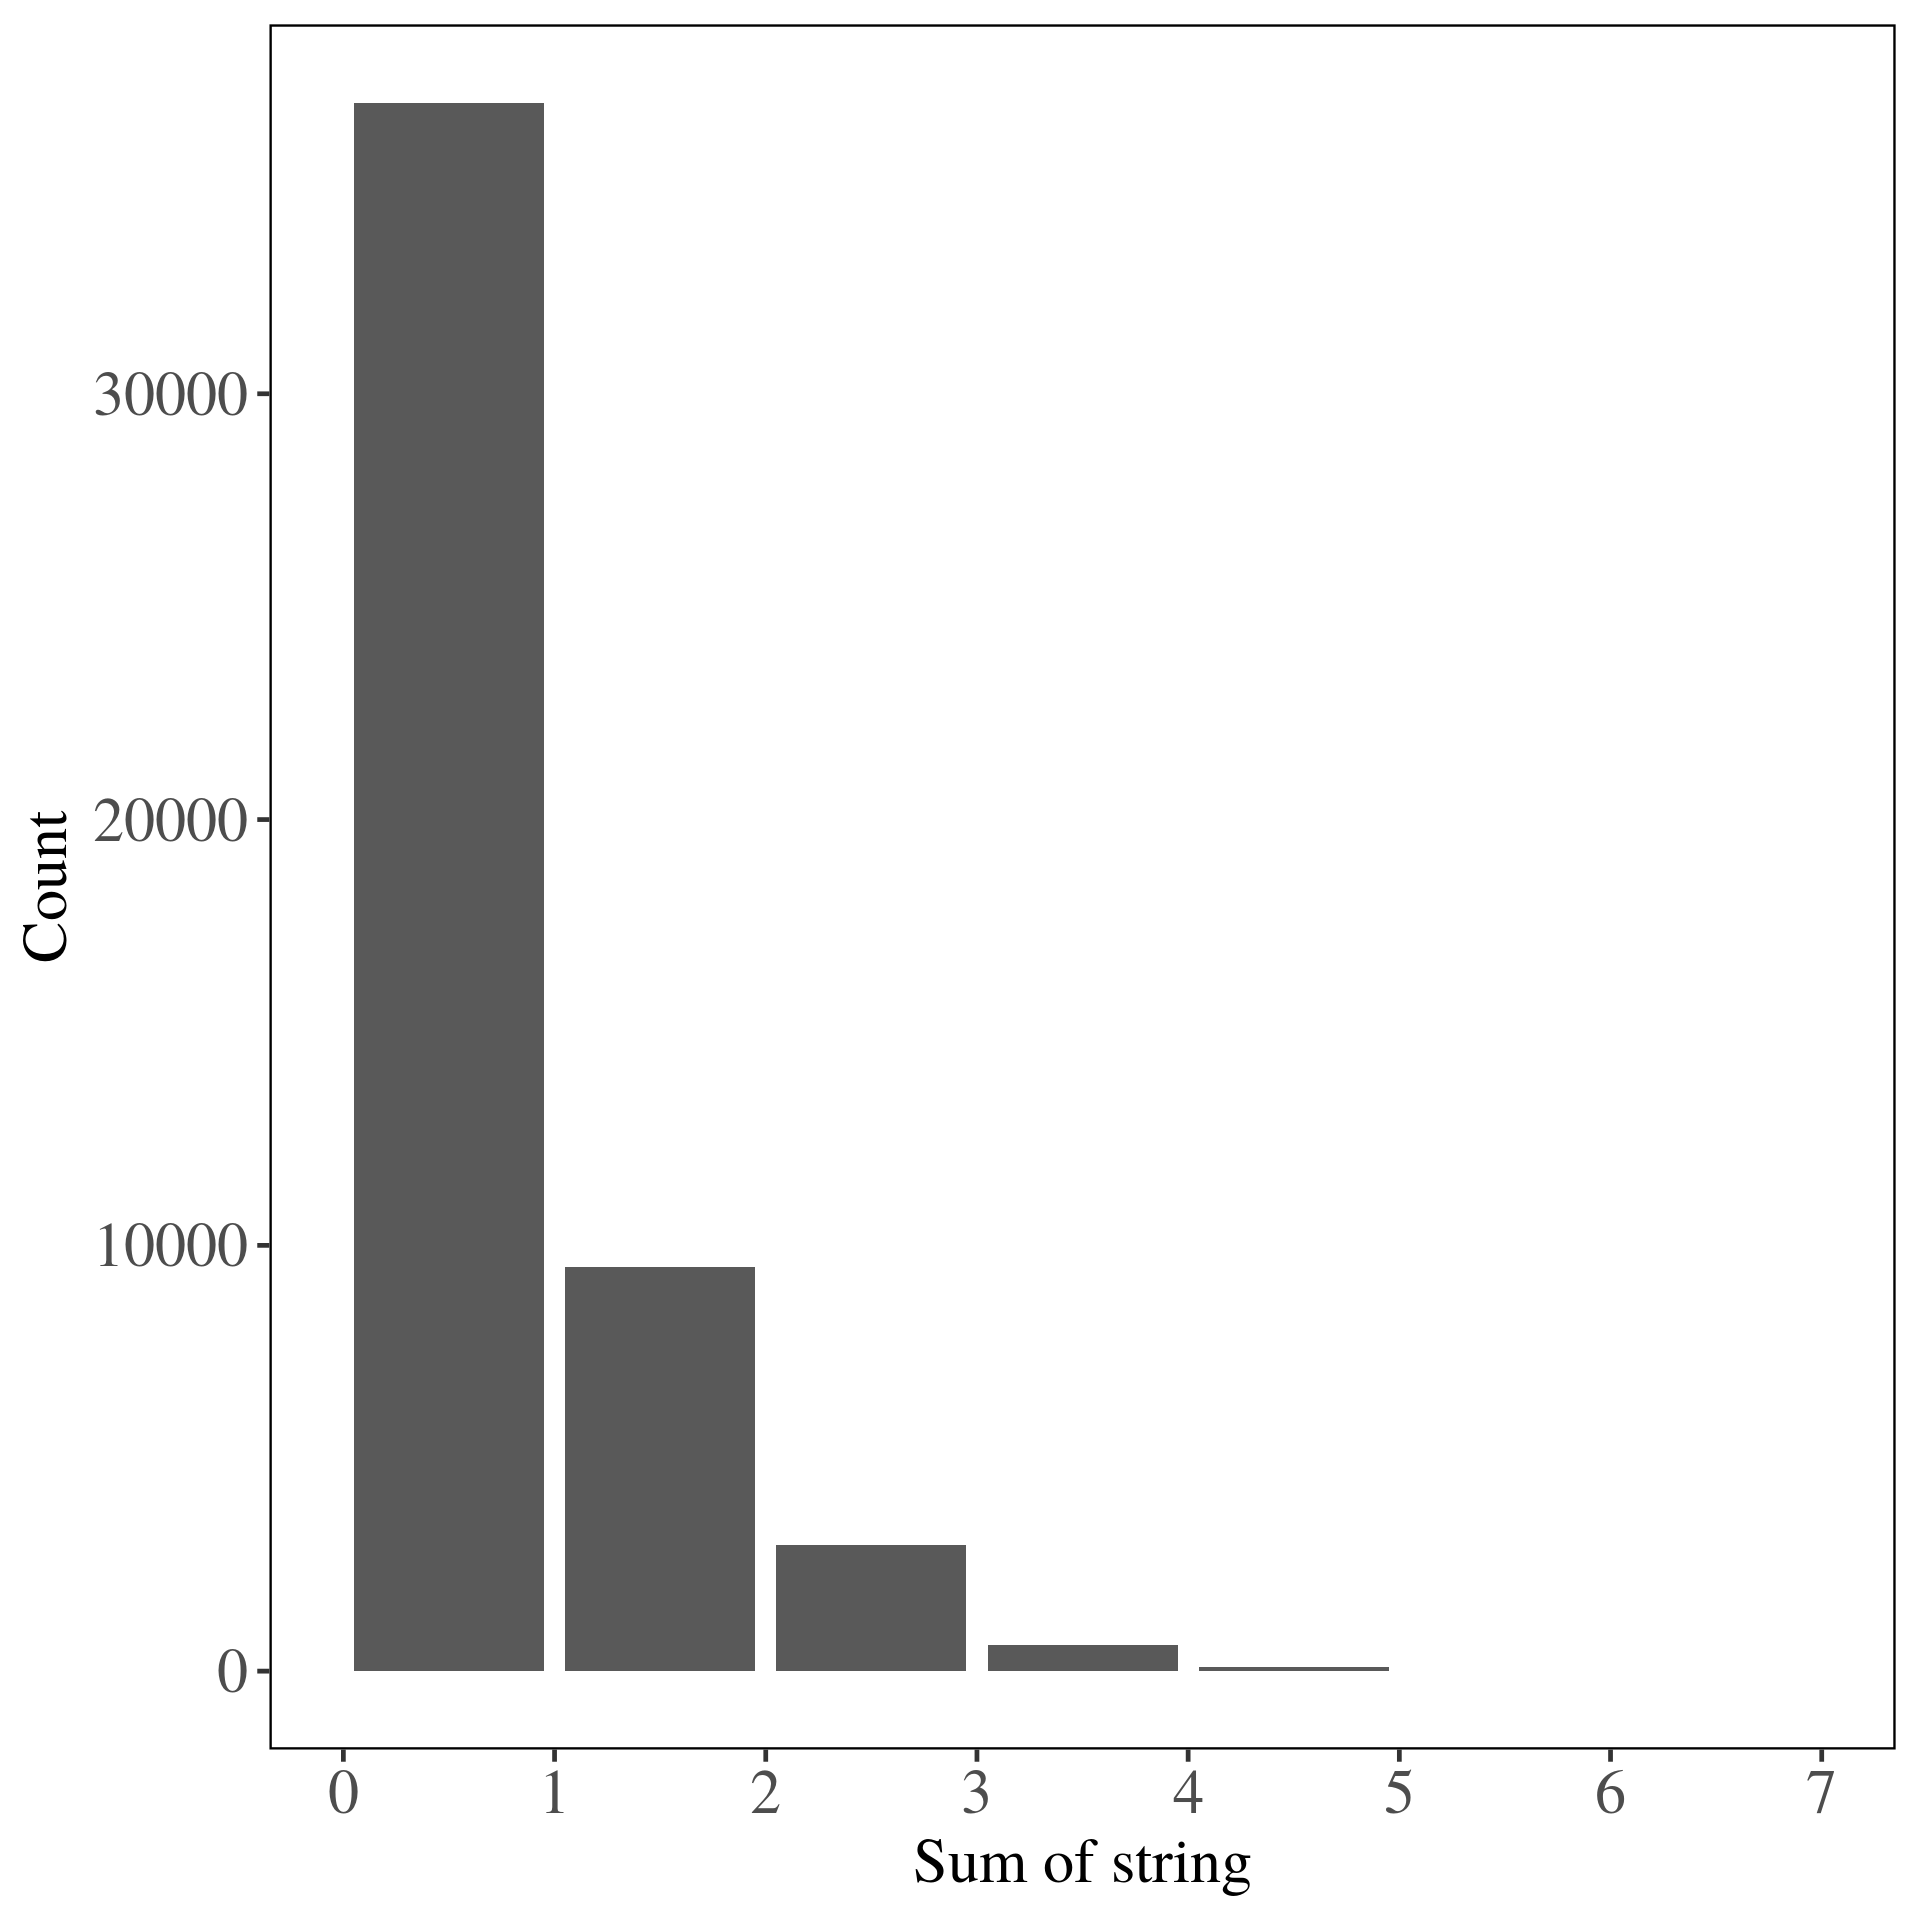
\includegraphics[width=1\linewidth]{img/sum_bp} 

}

\caption{Mjög áhugaverð mynd.}\label{fig:sumplt}
\end{figure}

\hypertarget{umruxe6uxf0a}{%
\subsection{Umræða}\label{umruxe6uxf0a}}

Tekur enga stund að keyra þessa skrá. Ef það þarf að breyta myndum eða töflum er það gert í \texttt{binomial\_wrangl.R} og svo endurprjóna \texttt{index.Rmd}. Allar tölur eru birtar með vísum í minni svo það þarf ekki að endurskrifa neinar tölur. Hef notað þessa uppsetningu til að skila heimadæmum og skýrslum í áföngum eins og Hagnýt Bayesísk tölfræði og Stærðfræðigreining IV þar sem það þurfti að blanda saman kóða, töflum, myndum og stærðfræði. Dæmi um stærðfræði:

\[
\mbox{Ei}(x) = -\int _{-x} ^{\infty} \frac{e^{-t}}{t} dt.
\]

\newpage

\hypertarget{kuxf3uxf0i}{%
\section{Kóði}\label{kuxf3uxf0i}}

\hypertarget{stillingarskruxe1-settings.r}{%
\subsection{Stillingarskrá: settings.R}\label{stillingarskruxe1-settings.r}}

\begin{Shaded}
\begin{Highlighting}[]
\KeywordTok{library}\NormalTok{(tidyverse)}
\KeywordTok{library}\NormalTok{(gridExtra)}
\KeywordTok{library}\NormalTok{(ggthemes)}
\KeywordTok{library}\NormalTok{(ggpubr)}
\KeywordTok{library}\NormalTok{(knitr)}
\KeywordTok{library}\NormalTok{(kableExtra)}
\KeywordTok{library}\NormalTok{(latex2exp)}
\KeywordTok{library}\NormalTok{(bookdown)}
\KeywordTok{library}\NormalTok{(scales)}
\KeywordTok{theme_set}\NormalTok{(}\KeywordTok{theme_tufte}\NormalTok{() }\OperatorTok{+}
\StringTok{            }\KeywordTok{theme}\NormalTok{(}\DataTypeTok{panel.border =} \KeywordTok{element_rect}\NormalTok{(}\StringTok{'black'}\NormalTok{, }\DataTypeTok{fill =} \OtherTok{NA}\NormalTok{),}
                  \DataTypeTok{text =} \KeywordTok{element_text}\NormalTok{(}\DataTypeTok{size =} \DecValTok{14}\NormalTok{),}
                  \DataTypeTok{legend.text=}\KeywordTok{element_text}\NormalTok{(}\DataTypeTok{size=}\DecValTok{14}\NormalTok{),}
                  \DataTypeTok{axis.text=}\KeywordTok{element_text}\NormalTok{(}\DataTypeTok{size=}\DecValTok{14}\NormalTok{),}
                  \DataTypeTok{axis.title =} \KeywordTok{element_text}\NormalTok{(}\DataTypeTok{size =} \DecValTok{14}\NormalTok{),}
                  \DataTypeTok{plot.title =} \KeywordTok{element_text}\NormalTok{(}\DataTypeTok{hjust =} \FloatTok{0.5}\NormalTok{)))}

\KeywordTok{ifelse}\NormalTok{(}\KeywordTok{exists}\NormalTok{(}\StringTok{'d'}\NormalTok{), }\KeywordTok{print}\NormalTok{(}\StringTok{'Loaded'}\NormalTok{), d <-}\StringTok{ }\KeywordTok{read_csv}\NormalTok{(}\StringTok{'data/binom_sim.csv'}\NormalTok{))}
\end{Highlighting}
\end{Shaded}

\hypertarget{hermunarskruxe1-simulate_binomial.r}{%
\subsection{Hermunarskrá: simulate\_binomial.R}\label{hermunarskruxe1-simulate_binomial.r}}

\begin{Shaded}
\begin{Highlighting}[]
\KeywordTok{source}\NormalTok{(}\StringTok{'scripts/settings.R'}\NormalTok{)}
\CommentTok{#' Simulate bernoulli strings of length n with success probability p}
\CommentTok{#' and store strings with their sums in a data frame.}

\CommentTok{#' Initialize}
\NormalTok{n <-}\StringTok{ }\DecValTok{12}
\NormalTok{p <-}\StringTok{ }\DecValTok{1}\OperatorTok{/}\DecValTok{12}
\NormalTok{L <-}\StringTok{ }\FloatTok{5e4}
\NormalTok{bi_sim <-}\StringTok{ }\KeywordTok{data.frame}\NormalTok{(}\DataTypeTok{string =} \KeywordTok{character}\NormalTok{(),}
                     \DataTypeTok{sum =} \KeywordTok{numeric}\NormalTok{(),}
                     \DataTypeTok{stringsAsFactors =}\NormalTok{ F)}
\KeywordTok{set.seed}\NormalTok{(}\DecValTok{123}\NormalTok{)}
\CommentTok{#' Populate data frame}
\CommentTok{#' for loops are SLOW in R so this will run slowly (on purpose)}
\ControlFlowTok{for}\NormalTok{(i }\ControlFlowTok{in} \DecValTok{1}\OperatorTok{:}\NormalTok{L) \{}
\NormalTok{  string <-}\StringTok{ }\KeywordTok{rbinom}\NormalTok{(n, }\DecValTok{1}\NormalTok{, p)}
\NormalTok{  bi_sim[i, }\DecValTok{1}\NormalTok{] <-}\StringTok{ }\KeywordTok{paste}\NormalTok{(}\KeywordTok{as.character}\NormalTok{(string), }\DataTypeTok{collapse =} \StringTok{''}\NormalTok{)}
\NormalTok{  bi_sim[i, }\DecValTok{2}\NormalTok{] <-}\StringTok{ }\KeywordTok{sum}\NormalTok{(string)}
  \ControlFlowTok{if}\NormalTok{ (i }\OperatorTok\StringTok{ }\DecValTok{1000} \OperatorTok{==}\StringTok{ }\DecValTok{0}\NormalTok{) \{}
    \KeywordTok{print}\NormalTok{(i)}
\NormalTok{  \}}
\NormalTok{\}}

\CommentTok{# Export data }
\KeywordTok{write_csv}\NormalTok{(}\DataTypeTok{x =}\NormalTok{ bi_sim, }\DataTypeTok{path =} \StringTok{'data/binom_sim.csv'}\NormalTok{)}
\end{Highlighting}
\end{Shaded}

\hypertarget{gagnavinnsluskruxe1-binomial_wrangl.r}{%
\subsection{Gagnavinnsluskrá: binomial\_wrangl.R}\label{gagnavinnsluskruxe1-binomial_wrangl.r}}

\begin{Shaded}
\begin{Highlighting}[]
\KeywordTok{source}\NormalTok{(}\StringTok{'scripts/settings.R'}\NormalTok{)}
\NormalTok{d <-}\StringTok{ }\KeywordTok{read_csv}\NormalTok{(}\StringTok{'data/binom_sim.csv'}\NormalTok{)}

\CommentTok{# Plot barplot of sum}
\KeywordTok{ggplot}\NormalTok{(}\DataTypeTok{data =}\NormalTok{ d, }\KeywordTok{aes}\NormalTok{(}\DataTypeTok{x =}\NormalTok{ sum)) }\OperatorTok{+}
\StringTok{  }\KeywordTok{geom_bar}\NormalTok{() }\OperatorTok{+}
\StringTok{  }\KeywordTok{labs}\NormalTok{(}\DataTypeTok{x =} \StringTok{'Sum of string'}\NormalTok{,}
       \DataTypeTok{y =} \StringTok{'Count'}\NormalTok{) ->}\StringTok{ }\NormalTok{sum_bp}
\CommentTok{# Export plot}
\KeywordTok{ggsave}\NormalTok{(}\DataTypeTok{filename =} \StringTok{'img/sum_bp.png'}\NormalTok{, }\DataTypeTok{plot =}\NormalTok{ sum_bp,}
       \DataTypeTok{width =} \DecValTok{6}\NormalTok{, }\DataTypeTok{height =} \DecValTok{6}\NormalTok{, }\DataTypeTok{dpi =} \DecValTok{320}\NormalTok{)}

\CommentTok{# Get 10 most popular strings and their proportion}
\NormalTok{d }\OperatorTok
\StringTok{  }\KeywordTok{group_by}\NormalTok{(string) }\OperatorTok
\StringTok{  }\KeywordTok{summarize}\NormalTok{(}\DataTypeTok{p =} \KeywordTok{n}\NormalTok{()}\OperatorTok{/}\KeywordTok{nrow}\NormalTok{(d)) }\OperatorTok
\StringTok{  }\KeywordTok{arrange}\NormalTok{(}\KeywordTok{desc}\NormalTok{(p)) }\OperatorTok
\StringTok{  }\KeywordTok{ungroup}\NormalTok{() }\OperatorTok
\StringTok{  }\KeywordTok{filter}\NormalTok{(}\KeywordTok{row_number}\NormalTok{() }\OperatorTok{<=}\StringTok{ }\DecValTok{10}\NormalTok{) ->}\StringTok{ }\NormalTok{pop_strings}
\CommentTok{# Export data}
\KeywordTok{write_csv}\NormalTok{(}\DataTypeTok{x =}\NormalTok{ pop_strings, }\StringTok{'tables/pop_strings.csv'}\NormalTok{)}

\CommentTok{# Plot proprtions for pop_strings}
\KeywordTok{ggplot}\NormalTok{(}\DataTypeTok{data =}\NormalTok{ pop_strings, }\KeywordTok{aes}\NormalTok{(}\DataTypeTok{x =}\NormalTok{ string, }\DataTypeTok{y =}\NormalTok{ p, }\DataTypeTok{group =} \DecValTok{1}\NormalTok{)) }\OperatorTok{+}
\StringTok{  }\KeywordTok{geom_point}\NormalTok{() }\OperatorTok{+}
\StringTok{  }\KeywordTok{geom_line}\NormalTok{(}\DataTypeTok{size =} \DecValTok{1}\NormalTok{, }\DataTypeTok{color =} \StringTok{'red'}\NormalTok{, }\DataTypeTok{lty =} \DecValTok{2}\NormalTok{) }\OperatorTok{+}
\StringTok{  }\KeywordTok{labs}\NormalTok{(}\DataTypeTok{x =} \StringTok{'Binary string'}\NormalTok{,}
       \DataTypeTok{y =} \StringTok{'Proportion'}\NormalTok{) }\OperatorTok{+}
\StringTok{  }\KeywordTok{theme}\NormalTok{(}\DataTypeTok{axis.text.x =} \KeywordTok{element_text}\NormalTok{(}\DataTypeTok{angle =} \DecValTok{45}\NormalTok{, }\DataTypeTok{hjust =} \DecValTok{1}\NormalTok{)) ->}\StringTok{ }\NormalTok{prop_plt}
\CommentTok{# Export}
\KeywordTok{ggsave}\NormalTok{(}\DataTypeTok{filename =} \StringTok{'img/prop_plt.png'}\NormalTok{, }\DataTypeTok{plot =}\NormalTok{ prop_plt,}
       \DataTypeTok{width =} \DecValTok{6}\NormalTok{, }\DataTypeTok{height =} \DecValTok{6}\NormalTok{, }\DataTypeTok{dpi =} \DecValTok{320}\NormalTok{)}
\end{Highlighting}
\end{Shaded}

\end{document}
